\documentclass{article}
\usepackage[shortlabels]{enumitem}
\usepackage{amsmath}
\usepackage{graphicx}
\usepackage{placeins}
\usepackage{caption}
\usepackage{subcaption}
\usepackage{amsthm}

\begin{document}
\title{Image Feature Analysis}
\author{Nicolas Langley 904433991}
\maketitle
\section{Introduction}

This project looks to perform analysis of image characteristics using a Convolutional
Neural Network in order to identify specific image features.  

\section{Dataset Overview}

An overview of the datasets used in this project will be presented as follows:
\begin{enumerate}
  \item Dataset Contents
  \item Dataset Origins
  \item Relevance to Project
\end{enumerate}

\subsection{MNIST Dataset}

\begin{enumerate}
  \item The MNIST dataset contains a large number of handwritten digits. It contains 50,000 training
        examples as well as 10,000 testing samples. Each of the samples is a single handwritten digit
        from 0 to 9 centered in a $28x28$ image. This centering is done by computing the center of mass
        of the pixels in the data and translating the image so this point is at the center of the $28x28$
        image. 
  \item The dataset is a subset of the a database compiled by the National Institute of Standards and Technology
        (NIST) comprised of handwritten digits by both Census Bureau Employees and High School students. The MNIST 
        dataset is a re-mixed subset where half of the training images and half of the testing images were taken 
        from each of the Census Bureau Employee and High School student sets respectively.
  \item This dataset is very commonly used as an initial dataset for the testing of different machine learning
        techniques. For this project, it was used as the initial dataset for testing the implementation of the
        convolutional neural network (CNN) approach used. It was also used in the testing of the PCA-based technique.
        For the purpose of working with the CNN, the training dataset was divided into both a training and a validation
        data set
        \FloatBarrier
        \begin{figure}
          \caption{Sample of the MNIST dataset}
          \centering
          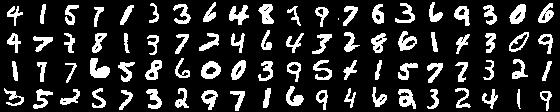
\includegraphics[scale=0.5]{images/mnist_dataset_example}
        \end{figure}
        \FloatBarrier
\end{enumerate}

\subsection{CIFAR Dataset}

\begin{enumerate}
  \item The CIFAR datasets are two datasets that contain a set of labelled $32x32$ color images. There are two
        versions of the dataset: one where the images are divided into 10 classes (CIFAR-10) and one where they are divided
        into 100 different classes (CIFAR-100). For this project, the CIFAR-100 dataset was used with a focus of the "coarse"
        labels provided (there are 20 coarse labels and 100 fine labels)
  \item These datasets are labelled subsets of the Tiny Images Dataset. The Tiny Images Dataset is a dataset of 80 million
        different $32x32$ images. The CIFAR datasets are comprised of a sampling of these images where the chosen images have
        been divided into classes and labelled.
  \item Within the context of this project, the CIFAR dataset was used as input to the Convolutional Neural Network as a more complex
        dataset than the MNIST dataset with real world (useful) classes that could be used in the identification process. A copy of the
        dataset was constructed where the images have been simplified by reducing their size to $28x28$ and converted to grayscale images.
        The images have also been whitened using PCA
        \FloatBarrier
        \begin{figure}
          \centering
          \begin{subfigure}{\textwidth}
            \centering
            \caption{Sample of original CIFAR dataset}
            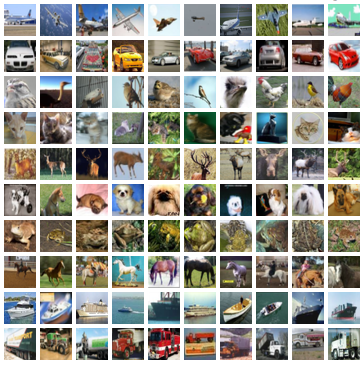
\includegraphics[scale=0.4]{images/cifar_dataset_example}
          \end{subfigure}
        \end{figure}
        \FloatBarrier
\end{enumerate}

\subsection{Custom Dataset}

\begin{enumerate}
  \item Test
\end{enumerate}

\section{Overview of Techniques}

This project involved the exploration of a number of techniques used to determine the features of an image. The technique that was settled
on and used for the attempted gathering of results was the Convolutional Neural Network. Other explored results were the use of Principal
Components Analysis on a set of images as well as simple MultiLayer Perceptrons and Logistic Regression. This report will go into detail on
the approach taken for testing each of these techniques as well as their results with respect to the goal of the project.

\subsection{Principal Components Analysis and Whitening}
  \subsubsection{Technique Overview}
  
  Principal Components Analysis (PCA) is a technique for converting a set of correlated variables into a set of linearly uncorrelated variables
  called Principal Components. The Principal Components are orthogonal to each other and starting with the first Principal Component, represent
  (in decreasing order) the largest possible variance. These Principal Components can be found by taking the eigendecomposition of the covariance
  matrix of a set of data. The Principal Components correspond to the eigenvectors of this decomposition.

  In this project, PCA was initially used as an approach for extracting the features of an image. This approach involves looking at a large set of
  like-images and extracting the Principal Components. These Principal Components will represent the areas of highest variance within the image and
  can be interpreted as being the features of the image set.
  
  PCA was used in preparation of the image data used as a part of the Whitening Transformation. The Whitening Transformation is a decorrelation
  transformation that transforms a set of random variables with a covariance matrix, $M$ into a set of random variables with the Identity matrix as
  their covariance matrix. This transformation serves to change the input vector into a white noise vector where all the random variables are decorrelated
  and their variance is 1. This transformation involves the following steps: \\
  \begin{enumerate}
    \item Given a data matrix $X_{k,n}$, center the data by subtracting the mean.
	\item Compute the covariance matrix $\Sigma = X X^{T} / n$
	\item Take the Eigenvalue Decomposition of $\Sigma$ to be $\Sigma = E D E^{T}$
	\item Re-arrange to get $D = E^{T} \Sigma E$
	\item Multiply the data $X$ by $D^{-\frac{1}{2}} E^{T}$ to get the 'whitened' data
  \end{enumerate}

  \subsubsection{Implementation}
  
  The implementation for this project was done in Python using a collection of scientific libraries. To see the implementation of the Whitening Transformation
  used in the project see the included source files

  \subsubsection{Results and Analysis}


\subsection{Logistic Regression}
  \subsubsection{Technique Overview}
  
  Logistic Regression is a basic probabilistic classification model. The purpose of the Logistic Regression technique is to predict the outcome of a class label
  based on a set of features. The classification process can be viewed as projecting an input vector onto a set of hyperplanes and determining the distance of the
  input to each hyperplane. The hyperplanes correspond to classes and distance of the input vector to any given hyperplane is used to determine the probability that
  the input matches the class defined by that hyperplane.

  The model takes as parameters a matrix $W$, which is a weight matrix, and $b$, which is a bias vector. With this information, the probability that an input vector 
  $x$ is a member of class $i$ is: \\
  \begin{align*}
  P(Y=i|x,W,b) &= \frac{e^{W_{i}x + b_{i}}}{\Sigma_{j}e^{W_{j}x + b_{j}}} \\
               &= softmax(Wx+b)
  \end{align*}
  The $softmax$ function transforms a $K$-dimensional vector of real values into a $K$-dimensional vector of real values in the range $[0 1]$ which represents a
  categorical probability distribution.
  
  Once the probability of the input belonging to any given class has been determined, the chosen class prediction is the class for which the highest probability
  was found i.e. $y_{pred} = max_{i}(P(Y=i|x,W,b))$ \\
  
  Using a Logistic Regression classifier involves training the parameters of the model using a training data set. Training is done by attempting to minimize a loss
  function. For this project, the negative log-likelihood was used as a measure of loss. Gradient descent is then used to generate the optimal parameters. Once a 
  model has been trained, it is possible to supply a test input vector and generate a predicted class label.
  
  \subsubsection{Implementation}
  
  Implementing a basic Logistic Regression classifier was done in Python using the Theano library. To see the code used, see the included source files

  \subsubsection{Results and Analysis}
  
  Using simply a basic Logistic Regression classifier resulted in classification of the MNIST dataset with  

\subsection{Multilayer Perceptron}

\subsection{Convolutional Neural Network}

\subsection{Other Approaches}

\section{Results and Further Work}

\section{Project Criterion Overview}

\end{document}
